\chapter{\label{chap:dataset}Obtaining Datasets for Self-Supervised Learning}

Datasets for self-supervised learning in general can be very different from each other, their form depends on the task that is being solved and the way of achieving the self-supervision. Although, all of them have one thing in common -- they mainly consist of unannotated data and at the end, they need smaller amount of annotated data to be able to classify from learned embeddings.

As is mentioned in Section~\ref{sec:self-supervised}, this thesis focuses on Time-Contrastive Learning (TCL), which means that it achieves supervision with multiple viewpoints of the same scene concurrently as is displayed in Figure~\ref{fig:scene-multiple-cameras}. While the filmed object may look very different when filmed from different angles, it is still the same object if the timestamps are identical. It is also possible to use moving cameras for filming of the scene, although this might introduce some inaccuracy to movement detection. On the other hand, even when the viewpoint is equivalent, the object can be altered only after a short time has passed. This characteristic holds supervision when TCL is used and because no extra work (e.g. labeling) has to be done, the data is supervised by itself -- self-supervised. The only restriction is the need to have multiple videos of the same scene synchronized in time.

\begin{figure*}[ht!]
    \centering

    \tikzstyle{scene} = [ellipse, minimum width=3cm, minimum height=2cm, text centered, draw=black]
    \tikzstyle{camera} = [rectangle, minimum width=2cm, minimum height=1cm, text centered, draw=black]
    \tikzstyle{arrow} = [thick,->,>=stealth]

    \begin{tikzpicture}[node distance=1.5cm]    
        \node (scene) [scene] {Scene};
        \node (cam2) [camera, below of=scene, yshift=-2cm] {Camera 2};        
        \node (cam1) [camera, left of=cam2, xshift=-2cm, yshift=1cm, rotate around={-50:(0,0)}] {Camera 1};
        \node (cam3) [camera, right of=scene, xshift=4cm, rotate around={90:(0,0)}] {Camera 3};

        \draw [arrow] (cam1) -- (scene);
        \draw [arrow] (cam2) -- (scene);
        \draw [arrow] (cam3) -- (scene);
    \end{tikzpicture}
    
    \caption{Example of a scene filmed from different viewpoints with 3 cameras. Higher number of viewpoints ensures greater variability in the dataset for time-contrastive learning.}
    \label{fig:scene-multiple-cameras}
\end{figure*}

It is necessary to have the process of dataset creation as automated as possible. Other\-wise it would have been easier to just label the data and simply use supervised learning approach. Therefore, I propose a set of tools in Section~\ref{sec:dataset-self-tool} that creates a dataset ready for TCL with just a small amount of user interaction. After that, a simple tool for labeling images is presented in Section~\ref{sec:dataset-label-tool}, because at least a small number of images with assigned class is always necessary.

At the end of this chapter, in Section~\ref{sec:dataset-sports-poses}, a basic dataset of sports poses is presented. It contains scenes with solid background and sports poses with variance only in arm movement and it was captured and prepared especially for this thesis. The basic sports pose dataset was demonstratively prepared only with tools described below. Finally, possible directions of development of dataset with advanced sports poses are discussed.

\section{\label{sec:dataset-self-tool}Creating Dataset for Time-Contrastive Learning}

Dataset for Time-Contrastive Learning (TCL) is created from synchronized videos of the same scene filmed from different angles. I propose a tool for semi-automatic preparation of such dataset, illustrated in Figure~\ref{fig:dataset-preparation}. It offers few simple editing features as cropping and trimming. Very important feature it provides is automatic synchronization of multiple videos. The second necessary component is a movement detector that estimates how much movement happened between frames of the video. This information is essential to achieve the time contrast that TCL relies on. Finally, the tool exports chosen video frames with their timestamps to simplify creating of triplets for model training.

\begin{figure*}[ht!]
    \centering

    \tikzset{diagonal fill/.style 2 args={
        fill=#1,
        path picture={
            \fill[#2, sharp corners] (path picture bounding box.south west) -| (path picture bounding box.north east) -- cycle;
        }
    }}
    \tikzstyle{io} = [rectangle, minimum width=1cm, minimum height=1cm,text centered, draw=black]
    \tikzstyle{manual} = [rectangle, minimum width=1.5cm, minimum height=1cm,text centered, draw=black, fill=red!30]
    \tikzstyle{semi} = [rectangle, minimum width=1.5cm, minimum height=1cm,text centered, draw=black, diagonal fill={red!30}{blue!30}]
    \tikzstyle{automatic} = [rectangle, minimum width=2cm, minimum height=1cm,text centered, draw=black, fill=blue!30]
    \tikzstyle{arrow} = [thick,->,>=stealth]

    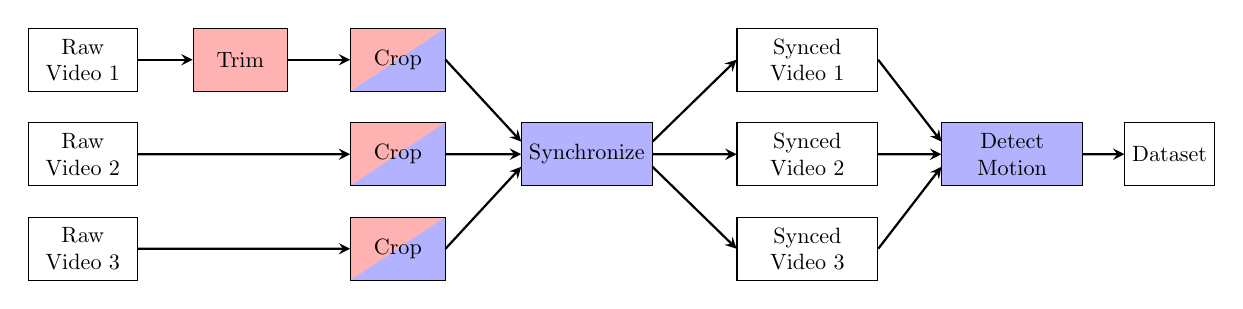
\begin{tikzpicture}[node distance=1.5cm, scale=0.8, every node/.style={scale=0.8}]    
        \node (input1) [io, text width=1.5cm] {Raw Video 1};
        \node (input2) [io, below of=input1, text width=1.5cm] {Raw Video 2};
        \node (input3) [io, below of=input2, text width=1.5cm] {Raw Video 3};

        \node (trim1) [manual, right of=input1, xshift=1cm] {Trim};
        
        \node (crop1) [semi, right of=trim1, xshift=1cm] {Crop};
        \node (crop2) [semi, below of=crop1] {Crop};
        \node (crop3) [semi, below of=crop2] {Crop};

        \node (sync) [automatic, right of=crop2, xshift=1.5cm] {Synchronize};

        \node (output1) [io, right of=sync, above of=sync, xshift=2cm, text width=2cm] {Synced Video 1};
        \node (output2) [io, below of=output1, text width=2cm] {Synced Video 2};
        \node (output3) [io, below of=output2, text width=2cm] {Synced Video 3};

        \node (motion) [automatic, right of=output2, xshift=1.75cm, text width=2cm] {Detect Motion};

        \node (dataset) [io, right of=motion, xshift=1cm] {Dataset};

        \draw [arrow] (input1) -- (trim1);

        \draw [arrow] (trim1) -- (crop1);
        \draw [arrow] (input2) -- (crop2);
        \draw [arrow] (input3) -- (crop3);

        \draw [arrow] (crop1.east) -- ([yshift=0.2 cm]sync.west);
        \draw [arrow] (crop2.east) -- (sync.west);
        \draw [arrow] (crop3.east) -- ([yshift=-0.2 cm]sync.west);

        \draw [arrow] ([yshift=0.2 cm]sync.east) -- (output1.west);
        \draw [arrow] (sync) -- (output2);
        \draw [arrow] ([yshift=-0.2 cm]sync.east) -- (output3.west);

        \draw [arrow] (output1.east) -- ([yshift=0.2 cm]motion.west);
        \draw [arrow] (output2.east) -- (motion.west);
        \draw [arrow] (output3.east) -- ([yshift=-0.2 cm]motion.west);
        
        \draw [arrow] (motion) -- (dataset);
    \end{tikzpicture}
    
    \caption{Tools for construction of dataset presented in the order of their usage. White boxes represent data and colored boxes the tools. Red color symbolizes tools that need some user interaction whereas blue colored tools are fully automatic. Tool for cropping needs a user to select a specific area but then it automatically adjusts the selection to fit all needs.}
    \label{fig:dataset-preparation}
\end{figure*}

Cross-platform video conversion solution \texttt{FFmpeg} is used to handle all video modifications effectively. Videos can be either processed directly with \texttt{FFmpeg} or a script is created that does the identical operations but can be launched later. The individual parts of the editing tool are presented in the following subsections in the order of their execution.

\subsection{Preparing Videos Filmed with Various Cameras}

The first step in dataset preparation is to trim the start and the end of the video. It is almost certain that the video contains a little bit of inapplicable footage at the beginning and at the end. Therefore, a simple tool that allows user to select the trim range with sliders is developed for the purpose of this thesis. Because of how the synchronization tool works, user only needs to trim one of the videos, the others will be trimmed automatically when being synchronized. This is further described in Section~\ref{sec:dataset-sync}.

In most cases, the video's resolution does not match the input of the model and has to be scaled down and is often also cropped to correct ratio. The tool allows user to select a bounding box around the scene which will always be included in the cropped video and non-important parts of the scene will mostly be deleted. Correct crop coordinates are automatically computed to match the input of the network and all other constraints. The computation consists of operations shown in Figure~\ref{fig:dataset-crop-process} and described into detail in the following enumerated list, their order is important.

\begin{enumerate}
    \item A view of the video as a single image is constructed from 10 merged frames taken out of the whole video in order to provide user with enough information about the range of motion.
    \item User selects the part of the scene that has to be included in the cropped video with a bounding box, these are the initial crop coordinates.
    \item Crop coordinates are adjusted to match the $height \times width$ ratio of the model input.
    \item If crop selection has lower resolution than the network input, the selection is equally extended.
    \item If crop selection exceeds the frame size, it is decreased to the closest possible value.
    \item If crop selection is positioned out of the frame, it is moved to the closest correct position.
    \item Video is cropped to the computed crop selection.
\end{enumerate}

\begin{figure*}[ht]\centering
    \centering
    \includegraphics[scale=0.5]{figures/dataset_crop/fig1.ai}
    \caption{Process of cropping a video with semi-automatic tool. User selects an area of interest with a bounding box and the tool performs cropping and resizing to a given resolution. The numbering of individual steps refers to previously mentioned description of the tool. Blue arrows symbolize automatic steps and red arrow a manual step. Steps 5 and 6 are only needed for some specific cases displayed in the figure, step 4 is not shown.}
    \label{fig:dataset-crop-process}
\end{figure*}

Crop coordinates are correctly computed to match the model input $height \times width$ ratio but the resolution will most likely not match. Therefore, the video has to be scaled down or (in case of video having lower resolution than model input) scaled up. Lastly, framerate of all of the videos has to be unified to a previously chosen fixed value to ensure correct run of synchronization and motion detection algorithms.

\subsection{\label{sec:dataset-sync}Synchronizing Videos by using Dense Optical Flow}

The main requirement for TCL to work is synchronization of all used videos. It is very likely that not all used videos are perfectly synchronized and manual synchronization would not be very precise nor effortless. Therefore, I present an automatic tool that determines the correct synchronization and trims all videos at the beginning and at the end so that all are the same length and are synchronized.

The synchronization is done by dense optical flow, which is information about the movement of each pixel between video frames \cite{HORN1981185}. Visualization of dense optical flow is shown in Figure~\ref{fig:optical-flow}. The assumption behind using dense optical flow for synchronization is that videos of the same scene have correlative amount of movement in similar directions at the same time. The precise movement of each pixel cannot be easily computed, it is only possible to approximate it. However, the precise values are not necessary for synchronization purposes, rough values are accurate enough.

\begin{figure*}[!ht]
    \begin{subfigure}[b]{0.24\textwidth}
        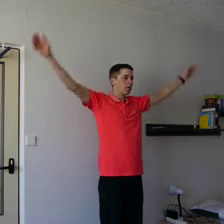
\includegraphics[width=\linewidth]{figures/optical_flow/frame000000312.png}
    \end{subfigure}
    \begin{subfigure}[b]{0.24\textwidth}
        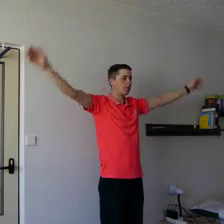
\includegraphics[width=\linewidth]{figures/optical_flow/frame000000386.png}
    \end{subfigure}
    \begin{subfigure}[b]{0.24\textwidth}
        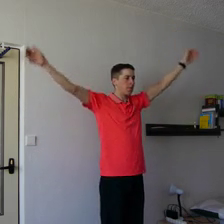
\includegraphics[width=\linewidth]{figures/optical_flow/frame000001127.png}
    \end{subfigure}
    \begin{subfigure}[b]{0.24\textwidth}
        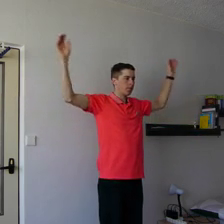
\includegraphics[width=\linewidth]{figures/optical_flow/frame000001664.png}
    \end{subfigure}
    \begin{subfigure}[b]{0.244\textwidth}
        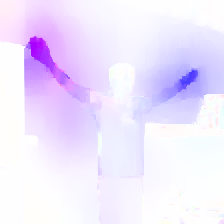
\includegraphics[width=\linewidth]{figures/optical_flow/flow000000312.png}
        \caption{}
        \label{fig:optical-flow-a}
    \end{subfigure}
    \begin{subfigure}[b]{0.244\textwidth}
        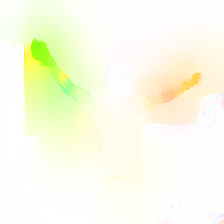
\includegraphics[width=\linewidth]{figures/optical_flow/flow000000386.png}
        \caption{}
        \label{fig:optical-flow-b}
    \end{subfigure}
    \begin{subfigure}[b]{0.244\textwidth}
        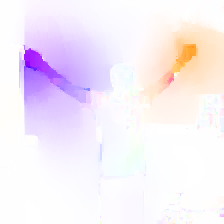
\includegraphics[width=\linewidth]{figures/optical_flow/flow000001127.png}
        \caption{}
        \label{fig:optical-flow-c}
    \end{subfigure}
    \begin{subfigure}[b]{0.244\textwidth}
        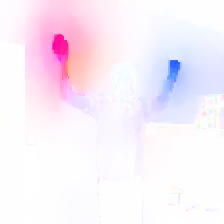
\includegraphics[width=\linewidth]{figures/optical_flow/flow000001664.png}
        \caption{}
        \label{fig:optical-flow-d}
    \end{subfigure}
    \caption{Dense Optical Flow visualized on multiple frames from the same video where a person is moving his arms. Visualization \ref{fig:optical-flow-a} shows both arms moving up while \ref{fig:optical-flow-b} captures both arms moving down. As can be deduced, visualization \ref{fig:optical-flow-c} is a combination of the previous two -- one arm is moving up and the other one down. Graphics \ref{fig:optical-flow-d} displays only forearms moving closer to each other while the elbows stay in place. All other parts of the frames stay steady.}
    \label{fig:optical-flow}
\end{figure*}

Movement vector of each pixel is from two reasons too specific for this task. First reason is that each video displays the scene from different angle and their optical flows will most likely be different. It is more useful to have general information about movement in the whole frame than to have it pixel-wise to eliminate small discrepancies. The second reason to aggregate information over the whole frame is growing computational complexity. If the information is accumulated over all pixels into a fixed number of values, the computational complexity stays constant, whereas it grows when pixel motion values are used individually. 

Since all pixels can move in two dimensions, it would make sense to gather information about horizontal and vertical movement by simply summing up all the values. Problem with this approach is that when some pixels move to the right and some to the left, their movement vectors subtract from each other in that dimension and a lot of information is lost. For that reason, I propose to sum separately positive and negative values in each dimension and obtain information about amount of motion in 4 directions -- up, down, left, and right. Each frame (except the first one) of each video is assigned these 4 values describing the optical flow from the previous frame to the current one.

After that, Pearson correlation of the aggregated optical flows of video pairs has to be done. These are not computed for all pair combinations, all flows are only compared to the shortest one to perform a smaller number of computations but still guarantee to get the best possible synchronization. Each flow pair is compared to get overlap with the highest correlation, that means correlation for each possible overlap is computed. Only restriction is that the overlap has to be at least a certain number of frames long to eliminate corner cases where for example only one frame has the best correlation (the first frame from one video and the last one from another). This minimal overlap length can be a little lower than what the expected length of synchronized videos is to optimize for the lowest number of correlations that has to be done. By default, it is set to $1{,}000$ frames.

Each overlap is assigned a specific index that will be used to describe it in the following text. The problem is that overlap index with the highest correlation might not be the correct one that synchronizes the videos because of some inaccuracy. To eliminate this problem, one additional property can be used -- if the correlations are computed accurately, the highest ones will be of overlap indices from similar range, just a few frames apart. To use this property, overlap indices are sorted descending by correlation and top 10 are taken. Standard deviation of these samples is computed and if it exceeds 10, it means that there is at least one overlap index among them that does not fit the majority. All these indices are checked and if they are further than one standard deviation from the mean, they are removed from this list. This operation is repeated until the standard deviation of the whole list is lower than 10. After that, the index with the highest correlation that is still in the list is the best one for synchronization. Real data example of this algorithm is provided in Table~\ref{tab:correlation-pick}.

\begin{table}[!ht]
    \begin{center}
        \begin{tabular}{ |c|c|c|c| }
            \hline
            State & \makecell{Best overlap indices \\ (descending by correlation)} & \makecell{Standard \\ deviation (SD)} & Allowed range \\
            \hline
            \hline
                Initial & \makecell{\textcolor{red}{2882}, 1410, 1543, 1692, 1691,\\1693, 1690, 1694, 1388, 1695} & \textcolor{red}{$398.7 > 10$} & $(1339, 2137)$ \\
            \hline
                1st epoch & \makecell{\textcolor{red}{1410}, 1543, 1692, 1691, 1693,\\1690, 1694, \textcolor{red}{1388}, 1695} & \textcolor{red}{$122.3 > 10$} & $(1488, 1733)$ \\
            \hline
                2nd epoch & \makecell{\textcolor{red}{1543}, 1692, 1691, 1693, 1690,\\1694, 1695} & \textcolor{red}{$52.3 > 10$} & $(1618, 1724)$ \\
            \hline
                3rd epoch & \makecell{\textcolor{green}{1692}, 1691, 1693, 1690, 1694,\\1695} & \textcolor{green}{$1.7 \mathrel{\ooalign{$>$\cr\hidewidth$|$\hidewidth}} 10$} & \makecell{Any -- SD \\ condition satisfied} \\
            \hline
        \end{tabular}
    \end{center}
    \caption{Example of real data from algorithm that tries to find the correct overlap index of two flows to have them correlated as much as possible. The algorithm needed 3 epochs to remove indices that had no other surrounding ones and, therefore, were detected as false findings. These indices are out of the allowed range, while the other were close to each other and in the allowed range. Index 1692 had the best correlation and was chosen as the best overlap index.}
    \label{tab:correlation-pick}
\end{table}

When the best overlap indices for the flow pairs are computed, flows are shortened to the same length where all of them overlapped. Their respective videos are trimmed at the beginning and at the end to have the same length as well and are thus synchronized because of the correct trim times.

\subsection{\label{sec:motion-detect}Detecting Movement with Sparse Optical Flow}

After videos of a scene are synchronized, the last step in creating the dataset is choosing the correct frames to be used for training of a neural network model. These frames have to satisfy one property -- there has to be enough movement between them for a model to be able to recognize the difference. The less movement is between the frames, the harder it will be for the model to learn embeddings of the filmed object but also the more precise the embeddings might be. It is necessary to set the movement threshold to a correct value since the dataset quality is crucial for the model's performance.

The first chosen approach was taking every $k$-th frame where $k$ was manually set by the amount of movement in the video. Since amount of movement varies in different timestamps of each video, this approach did not produce good enough frames for training. The next chosen tactics was using Dense Optical Flow for motion detection but this algorithm tracks every pixel in the video and the necessary information about movement of the followed object is lost in the amount of unnecessary data.

Therefore, I decided to use Sparse Optical Flow to fulfill the movement detection task. Unlike the Dense Optical Flow, the sparse variant chooses only some pixels with Shi-Tomasi corner detector and those are being tracked \cite{shi-tomasi-323794}. The amount of movement has to be ideally aggregated into a single number and summed frame after frame until it exceeds a certain threshold. Then, enough motion has been detected and the given frame is selected and motion detection continues again from zero to detect another frame. This procedure dynamically chooses the gap between chosen frames, which is essential for sports pose recognition. It is possible that at some times few seconds of no movement are followed with a lot of motion in just one second.

The challenging task is aggregating the information from sparse optical flow to a valuable metric. Since each scene can be different, the number of tracked pixels can also vary. Therefore, the distances cannot be easily summed but rather averaged. Another problem is introduced when the background of the scene is not solid and some of the tracked pixels are in the background. Those do not move and they should not influence the average distance of pixel movement. This is solved by calculating average of only those pixels, whose movement is above a certain threshold.

One more problem that was encountered during the development of motion detection algorithm was vanishing of monitored pixels. After a higher amount of movement, the pixels detected to be followed might get lost and there are not enough pixels left to precisely detect motion. When this happens, Shi-Tomasi corner detector has to be run again to detect new pixels for the sparse optical flow.

The last feature that the motion detector uses to provide more accurate results is accounting only for unique moves. If all pixels move the same way, that means the scene has changed but the sports pose probably did not change at all. This problem also has to be addressed. The motion detector does so by computing a cosine similarity between all motion vectors produced by sparse optical flow and ignores those vectors that are too similar.

Detected frames from the video are saved as images and will be used for self-supervised learning of a neural network. The motion detection has to be run prior to the learning procedure to enable for shuffling of training data and also to make loading of dataset less computationally demanding.

\subsection{Building Triplets from Video Frames}

Neural network used in this thesis is trained with triplet loss function and, therefore, it has to be provided with 2 data samples of the same pose from a different viewpoint and 1 sample of a different pose from the same viewpoint as one of the previous two. The goal is to provide the network with batches of such triplets.

At first, file paths to the correct images are formed into triplets and then into batches. After that, file paths are replaced with images that they were pointing at. Dataset of batches of triplets is then shuffled and split into training and validation subsets. Before each epoch, the training subset is always shuffled again to provide for higher variability.

\subsection{\label{sec:dataset-label-tool}Tool for Labeling Sports Poses in Dataset}

Even though the main advantage of self-supervision is that very few annotated training samples are needed, there is still a need for some of them. That is why I decided to also develop a tool for very fast and easy labeling of training samples. This labeling tool takes a directory with unsorted images as an input and moves them to their respective directories named after their labels.

If launched for the first time, new classes have to be assigned to specific keyboard keys and then with just a single press of the key, displayed image is assigned to its class. This procedure makes image labeling as minimalistic as possible. Key-class pairs are saved as a dictionary to a file that can be loaded at anytime to continue with annotating of images.

\section{\label{sec:dataset-sports-poses}Dataset of Sports Pose Images}

Multiple sets of videos were recorded for developing of tools for dataset suitable for time-contrastive learning and then for the sports pose recognition itself. At first, the goal was to obtain dataset consisting of simple scene that presents an easy challenge for both the dataset preparing tools and for recognition models. Afterwards, a more difficult task can be presented to the dataset tools and encoding and classifying models, e.g. a dataset with sports poses recorded in multiple environments. Sports poses from yoga are proposed for future development as one of the most challenging tasks possible in this field.

\subsection{\label{sec:dataset-hand}Hand Poses as a Simple Testing Data}

One hand in different poses is a real world situation with pretty low variability, especially if the background is solid. Therefore, it is a good candidate for testing data for the dataset preparation tools and can be used for the testing of a self-supervised trained model during its development. The original videos are cropped so that only forearm and hand with fingers is in the frame to make them as elementary as possible. This dataset will be referred to as the Hand Dataset. Examples of its images are shown in Figure~\ref{fig:dataset-hand-simple-example}.

\begin{figure*}[!ht]
    \centerline{
        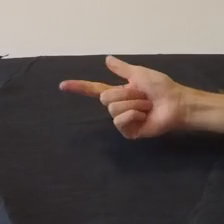
\includegraphics[scale=0.46]{figures/dataset_hand/scene003_cam2_image00025.png}
        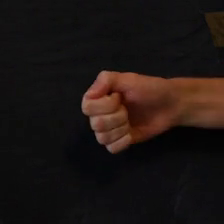
\includegraphics[scale=0.46]{figures/dataset_hand/scene004_cam0_image00015.png}
        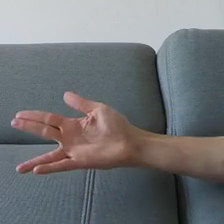
\includegraphics[scale=0.46]{figures/dataset_hand/scene005_cam2_image00080.png}
        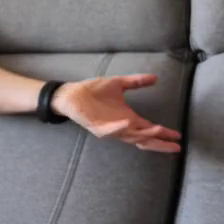
\includegraphics[scale=0.46]{figures/dataset_hand/scene006_cam1_image00033.png}
    }
    \vspace{0.1cm}
    \centerline{
        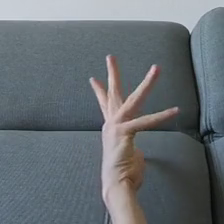
\includegraphics[scale=0.46]{figures/dataset_hand/scene007_cam2_image00028.png}
        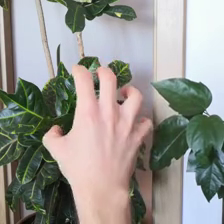
\includegraphics[scale=0.46]{figures/dataset_hand/scene008_cam1_image00024.png}
        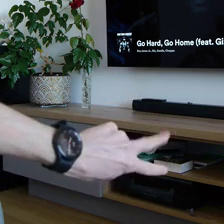
\includegraphics[scale=0.46]{figures/dataset_hand/scene009_cam0_image00010.png}
        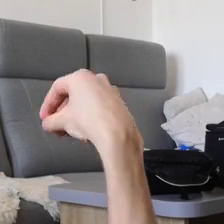
\includegraphics[scale=0.46]{figures/dataset_hand/scene010_cam1_image00019.png}
    }
    \caption{Hand Dataset images from different scenes. Some images have fairly solid background while the others have very heterogenous one to simulate various possible situations for the dataset preparation tools.}
    \label{fig:dataset-hand-simple-example}
\end{figure*}

Trimming and cropping of the video are done completely manually and basically are not dependent on the dataset, the first real challenge comes with the automatic synchronization of videos from multiple viewpoints. The task was easily fulfilled on videos with solid background and not so different viewpoints but once these two conditions were disrupted, an incorrect synchronization could be found. Therefore, an algorithm that searched for top 10 best synchronization timestamps, not only the best one, was developed. This algorithm is fully described in the previous section.

Following challenge was to obtain specific frames from the video used for training. Videos without a solid background showed the importance of only taking into account the moving pixels because the Shi-Tomasi corner detector used in Sparse Optical Flow computation selects also pixels from the background, not only those related to the followed object. Another task that this dataset exposed was vanishing of the followed pixels. The last and most difficult challenge to solve was detection of translation where the pose actually does not change. Movement without any pose adjustment is a phenomenon normally present in this dataset. Another instance of the same problem is when the camera is moving and the pose stays in the same position.

\subsection{\label{sec:dataset-upper-body}Sports Poses with Upper Body Movement}

The Hand Dataset served its purpose in making of the dataset preparation tools and the next task is the development of the self-supervised model. I recorded and prepared a dataset of simplified sports poses that are less complicated than what would for example yoga poses look like but still have the character of sports poses. Example of poses can be seen in Figure~\ref{fig:dataset-upper-body-example}. All of the recorded poses hold these conditions. The person is recorded from knees up and moving only its arms, while any bending of shoulders, elbows, wrists, and fingers is allowed (and advised).

\begin{figure*}[!ht]
    \centerline{
        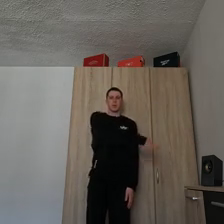
\includegraphics[scale=0.46]{figures/dataset_upper_body/scene026_cam1_image00169.png}
        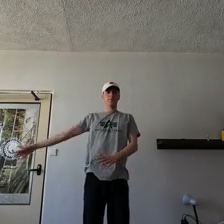
\includegraphics[scale=0.46]{figures/dataset_upper_body/scene024_cam1_image00077.png}
        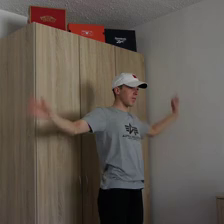
\includegraphics[scale=0.46]{figures/dataset_upper_body/scene025_cam0_image00037.png}
        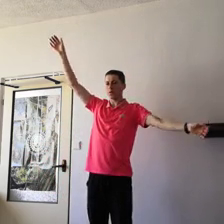
\includegraphics[scale=0.46]{figures/dataset_upper_body/scene020_cam2_image00019.png}
    }
    \vspace{0.1cm}
    \centerline{
        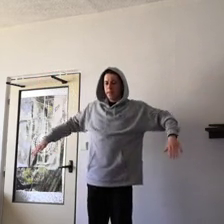
\includegraphics[scale=0.46]{figures/dataset_upper_body/scene022_cam2_image00066.png}
        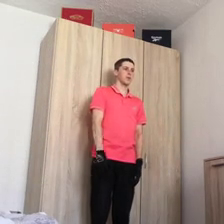
\includegraphics[scale=0.46]{figures/dataset_upper_body/scene029_cam2_image00153.png}
        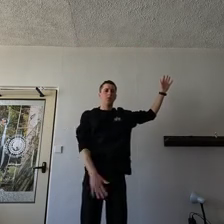
\includegraphics[scale=0.46]{figures/dataset_upper_body/scene023_cam1_image00006.png}
        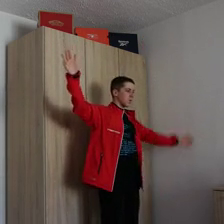
\includegraphics[scale=0.46]{figures/dataset_upper_body/scene028_cam0_image00224.png}
    }
    \centerline{
        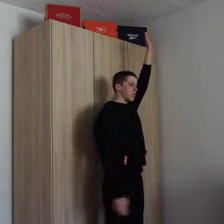
\includegraphics[scale=0.46]{figures/dataset_upper_body/scene026_cam0_image00182.png}
        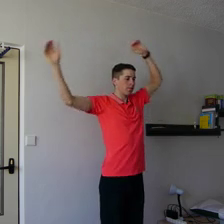
\includegraphics[scale=0.46]{figures/dataset_upper_body/scene020_cam0_image00026.png}
        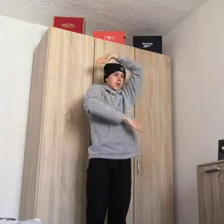
\includegraphics[scale=0.46]{figures/dataset_upper_body/scene027_cam2_image00022.png}
        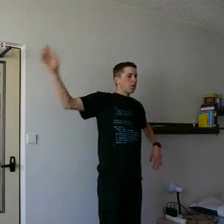
\includegraphics[scale=0.46]{figures/dataset_upper_body/scene021_cam0_image00006.png}
    }
    \vspace{0.1cm}
    \centerline{
        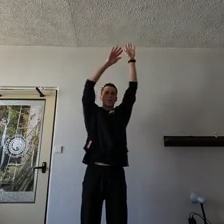
\includegraphics[scale=0.46]{figures/dataset_upper_body/scene023_cam1_image00035.png}
        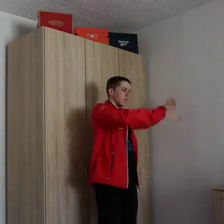
\includegraphics[scale=0.46]{figures/dataset_upper_body/scene028_cam0_image00247.png}
        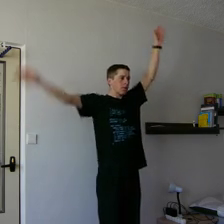
\includegraphics[scale=0.46]{figures/dataset_upper_body/scene021_cam0_image00044.png}
        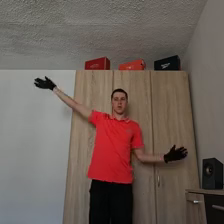
\includegraphics[scale=0.46]{figures/dataset_upper_body/scene029_cam1_image00142.png}
    }
    \caption{Samples from dataset with upper body poses. Recordings come from 2 places, each with 5 videos with different clothing. The scenes are recorded with 3 cameras from different viewpoints.}
    \label{fig:dataset-upper-body-example}
\end{figure*}

The dataset videos include one person in two scenes with different background. There are 5 recordings of each scene with the person wearing various clothing in each of them to increase variability in the dataset. That means 10 recordings in total. Performed poses are chosen randomly. Each scene was filmed with 3 cameras with different lenses. The camera angles were chosen so that one is facing straight from the front side and one is on each side in approximately 45 degrees angle from the front one. The total number of images in the dataset is $3{,}804$ but each of those is one of $1{,}268$ potentially different poses captured with 3 cameras. Distribution of the poses count across all ten recordings is following: 34, 49, 67, 99, 96, 51, 204, 128, 295, 245.

\subsection{\label{sec:dataset-labels}Sorting Upper Body Dataset into Classes}

The recorded dataset of arm movement is prepared for self-supervised training of an encoder model but for real recognition, some amount of labeled samples is also necessary. There are many different ways to sort all the poses into classes. I decided to assign two sets of labels to all the samples to have enough data for experiments, one with a lower number of classes that presents an easier recognition task and the other with higher number of classes to demonstrate the models performance.

At first, I divided the data into 4 classes to create an easier task. Since arms are the only moving entities in the image, only those are taken into account and the rest of the body is ignored. Each arm can be either in upward or downward direction but when various elbow bendings are taken into account, resolving whether arm is pointing up or down is ambiguous. Therefore, a strict criteria has to be set. I decided to use the height of wrist and shoulder to be the determining factor. If a wrist is above shoulder height, the arm is in upward position. Finally, each arm is dealt with separately and that means 4 classes emerge: both arms down (down-down -- $1{,}146$ samples), left arm down and right arm up (down-up -- 813 samples), left arm up and right arm down (up-down -- 795 samples) and both arms up (up-up -- $1{,}050$ samples). Dataset with basic sports poses divided into these 4 classes will be from now on referred to as Directions Dataset.

For more complex and convincing evaluation of developed models, I prepared one more set of labels with finer separation. The main thought is the same as for the Directions Dataset -- each arm is either pointing up or down, but one more feature was added. Each arm can be either bent in the elbow or not -- if the elbow angle is smaller than 135 degrees, arm is considered bent. All of the Directions Dataset classes have 2 possible options which creates 16 classes in total. Higher number of classes not only allows for more valuable testing of the model but also brings option of evaluating not only top-1 accuracy but also top-3 accuracy. When the correct class of a certain pose is not the one with the highest probability according to the classifier but still is the second or third, the model shown some ability to recognize poses too. Counts of samples for each class of the Bent Dataset are presented in Table~\ref{tab:bent-dataset-counts}. Class names are derived from the Directions Dataset, only change is that when an arm in the given direction is bent, letter `b' is placed in front of the direction.

\begin{table}[!ht]
    \footnotesize
    \begin{center}
        \begin{tabular}{ |c|c||c|c||c|c||c|c| }
            \hline
                Class & \makecell{Sample \\ count} & Class & \makecell{Sample \\ count} & Class & \makecell{Sample \\ count} & Class & \makecell{Sample \\ count} \\
            \hline
            \hline
            down-down & $1{,}005$ & bdown-down & $63$ & down-bdown & $48$ & bdown-bdown & $63$ \\
            \hline
            down-up & $399$ & bdown-up & $21$ & down-bup & $285$ & bdown-bup & $102$ \\
            \hline
            up-down & $399$ & bup-down & $282$ & up-bdown & $33$ & bup-bdown & $90$ \\
            \hline
            up-up & $495$ & bup-up & $135$ & up-bup & $99$ & bup-bup & $285$ \\
            \hline
        \end{tabular}
    \end{center}
    \caption{Distribution of sports pose images between all classes of the Bent Dataset. First word shows direction that the left arm is heading, second word represents the right arm. If the arm is bent, letter `b' precedes the direction.}
    \label{tab:bent-dataset-counts}
\end{table}

Both of the presented datasets cannot be perfectly divided into classes without any discrepancy. Followed features are in some cases right in between the available classes. Arm can be almost perfectly horizontal with its wrist in the same height as shoulder. Correspondingly, elbow angle can be precisely 45 degrees or very close to it and it is not possible to distinguish this difference from a single image. Therefore, some error rate is almost inevitable and has to be taken into account during the model evaluation.

Directions Dataset has fairly equally distributed images between classes whereas Bent Dataset has significant disproportions in the counts. This presents another challenge for classifier that is trying to learn on the data. In general, self-supervised models should have better performance on such data because they first learn the data embeddings without any labels and then solve fairly simple task in classifying those. In contrast to supervised classifier that is solving the difficult task directly on the labeled data and might not update its weights enough because other classes in the batch are more significant.

\subsection{Yoga Sports Poses for Future Development}

Yoga sports poses are one the most complex among all sports poses, there are hundreds of possible poses and their variants. They can be also sorted into different sets according to their similarities. All these attributes make them the perfect candidate for a very difficult sports pose recognition task and, therefore, I propose yoga poses as a benchmark for the future development in this field.

Verma et al. in \cite{verma2020yoga} present a new dataset Yoga-82 for human pose classification that is based on yoga poses. It contains over 28 400 annotated samples of 82 different yoga poses. The classes are sorted into 3-level hierarchy where each of the 82 poses are assigned a second and first-level class as well. This structure can be further used for recognition of poses that are projected into an embedding space since embeddings of poses from the same higher-level class can have similarities in the space.

The dataset is available to download in form of URL links to each image sorted into files according to their classes. The images are under different creative common licenses. There is no script for downloading of the images as a part of the publication. Since the images are from various sources from the internet, their availability is out of reach of the dataset authors. In the time of publishing this thesis, there are already hundreds of images not available.

The images differ in resolution and aspect ratio, therefore, some sort of preprocessing is necessary. Their variability is very high, they are captured both indoors and outdoors and with very different backgrounds. The displayed people differ in their gender, skin color, clothing, and other visible characters. Some images even contain multiple people, text added over the pose in postproduction or the images are just a simple illustration of the pose, not a real photo. These additional features might not serve well for better generalization of the trained model, rather for confusion because of the unrealism.

These images could be used for classification of the poses from embeddings but the more complicated task is learning the sports pose embeddings with a time-contrastive network. This process requires synchronized videos or at least images of the same scene from different viewpoints. I have not found such dataset online and therefore, I suspect it has to be recorded specifically for this task. One possible solution for making the dataset creation more feasible would be to partner with some yoga video producer. There is a chance they are filming their videos from multiple angles and could offer their raw recordings for such project. The variability of all recordings has to be taken into account. If they are from the same environment (e.g. indoor gym), the model will probably not generalize well to other surroundings (for example outdoors).
